\section{Highlighting Named Storms}

    To estimate the ability of the algorithm to accurately capture the length of a windstorm, we experiment by appending different lengths of time to the points identified as belonging to a storm over land and with wind speed above 20m/s, as discussed in Chapter 3.3.1. The results of these experiments are presented in Table \ref{tab:stormcat}, where the second column contains the number of hours appended before/after the point in the format X/Y. We also identify the period during which the five cyclones produce windstorms over land, which does not always match the defined start and end time of the storm. This is achieved through the Copernicus Extreme Winds Catalogue, which provides animations representing the movement of cyclones and the strength of winds in western Europe, as well as information on the start and end dates of the storms. We chose 4 named storms and 1 severe but unnamed one: the Great Storm of '87, Lothar, Kyrill, Emma and a storm on the 13th of January 1993. All of the above storms have caused considerable damage and high insurance loss. 

        \begin{table}
        \centering
        \resizebox{0.95\textwidth}{!}{%
        \begin{tabular}{llllll}
        Windstorm   &       & Start       & End         & Match & Extra Days \\ \hline
        Emma        & data  & 25 Feb 2008 & 05 Mar 2008 &       &            \\
                    & DWOL  & 28 Feb 2008 & 5 Mar 2008  &       &            \\
                    & 24/12 & 29 Feb      & 04 Mar      & 75\%  & 0          \\
                    & 24/24 & 29 Feb      & 07 Mar      & 75\%  & 2          \\
                    & 30/24 & 29 Feb      & 07 Mar      & 75\%  & 2          \\
                    & 30/30 & 29 Feb      & 08 Mar      & 75\%  & 3          \\
                    & 36/36 & 20 Feb      & 08 Mar      & 100\% & 6          \\ \hline
        13 Jan '93  & data  & 12 Jan 1993 & 16 Jan 1993 &       &            \\
                    & DWOL  & 12 Jan 1993 & 16 Jan 1993 &       &            \\
                    & 24/12 & 08 Jan      & 15 Jan      & 80\%  & 4          \\
                    & 24/24 & 08 Jan      & 15 Jan      & 80\%  & 4          \\
                    & 30/24 & 07 Jan      & 15 Jan      & 80\%  & 5          \\
                    & 30/30 & 07 Jan      & 15 Jan      & 80\%  & 5          \\
                    & 36/36 & 07 Jan      & 16 Jan      & 99\%  & 5          \\ \hline
        G.S. of '87 & data  & 14 Oct 1987 & 19 Oct 1987 &       &            \\
                    & DWOL  & 14 Oct 1987 & 19 Oct 1987 &       &            \\
                    & 24/12 & 13 Oct      & 16 Oct      & 50\%  & 0          \\
                    & 24/24 & 13 Oct      & 17 Oct      & 66\%  & 0          \\
                    & 30/24 & 13 Oct      & 17 Oct      & 66\%  & 0          \\
                    & 30/30 & 13 Oct      & 17 Oct      & 66\%  & 0          \\
                    & 36/36 & 13 Oct      & 17 Oct      & 67\%  & 0          \\ \hline
        Lothar      & data  & 23 Dec 1999 & 28 Dec 1999 &       &            \\
                    & DWOL  & 22 Dec 1999 & 29 Dec 1999 &       &            \\
                    & 24/12 & 22 Dec      & 28 Dec      & 88\%  & 0          \\
                    & 24/24 & 22 Dec      & 29 Dec      & 99\%  & 0          \\
                    & 30/24 & 21 Dec      & 29 Dec      & 100\% & 1          \\
                    & 30/30 & 21 Dec      & 29 Dec      & 100\% & 1          \\
                    & 36/36 & 21 Dec      & 29 Dec      & 100\% & 1          \\ \hline
        Kyrill      & data  & 16 Jan 2007 & 21 Jan 2007 &       &            \\
                    & DWOL  & 16 Jan 2007 & 21 Jan 2007 &       &            \\
                    & 24/12 & 17 Jan      & 19 Jan      & 50\%  & 0          \\
                    & 24/24 & 17 Jan      & 22 Jan      & 83\%  & 0          \\
                    & 30/24 & 17 Jan      & 22 Jan      & 83\%  & 0          \\
                    & 30/30 & 17 Jan      & 22 Jan      & 83\%  & 1          \\
                    & 36/36 & 08 Jan      & 25 Jan      & 100\% & 10        
        \end{tabular}%
        }
        \caption{The ability of the algorithm to encompass a windstorm event. The numbers in X/Y format in the second column represent the amount of hours appended before/after a point identified as belonging to a storm over land and of wind speed above 20m/s. Storm data extracted from the Copernicus Extreme Winds Catalogue. DWOL represents the Days a Windstorm is Over Land.}
        \label{tab:stormcat}
        \end{table}

    As the appended number of hours increases, we observe an improved match between the dates during which windstorms occur for an event and the dates computed by the algorithm for the event. However, we also experience a growing number of noisy days, which are days outside the range of a storm. In this study, we make use of the fifth option which appends 36 hours on both ends of datapoints and minimise the noise from additional days by implementing a secondary wind speed threshold of 15m/s, the aim of which is to filter out any nonviolent winds. This way, we hope to filter out additional days as they will most likely not pass this test. However, this introduces the risk of merging two separate storms into a singular event if they occur with little time inbetween.

\section{Estimating Loss}

    We evaluated the ability of the storm energy-based SSI, developed for this study, to estimate insurance loss and found that it shows low correlation with a list of 50 storms extracted from the Copernicus Extreme Windstorm Catalogue. It performs similarly to another meteorologically focused SSI used in industry and presented in detail in Chapter 2. The energy-based SSI has a p-value of 0.60, while the one used in industry has a slightly higher p-value of 0.66. The reason for the poor performance in estimating loss is that both methods do not consider variables describing the vulnerability to damage in the area over which computation is performed, such as population or an infrastructural development index. We present a scatter plot in Figure \ref{fig:scatterSSI} illustrating the performance of both indices. Both models severely underestimated the loss caused by the Great Storm of '87, which moves along the western coast of Europe, but by the time it passes over land and is detected by the algorithms, it has already caused considerable damage.
    
        \begin{figure}
            \centering
            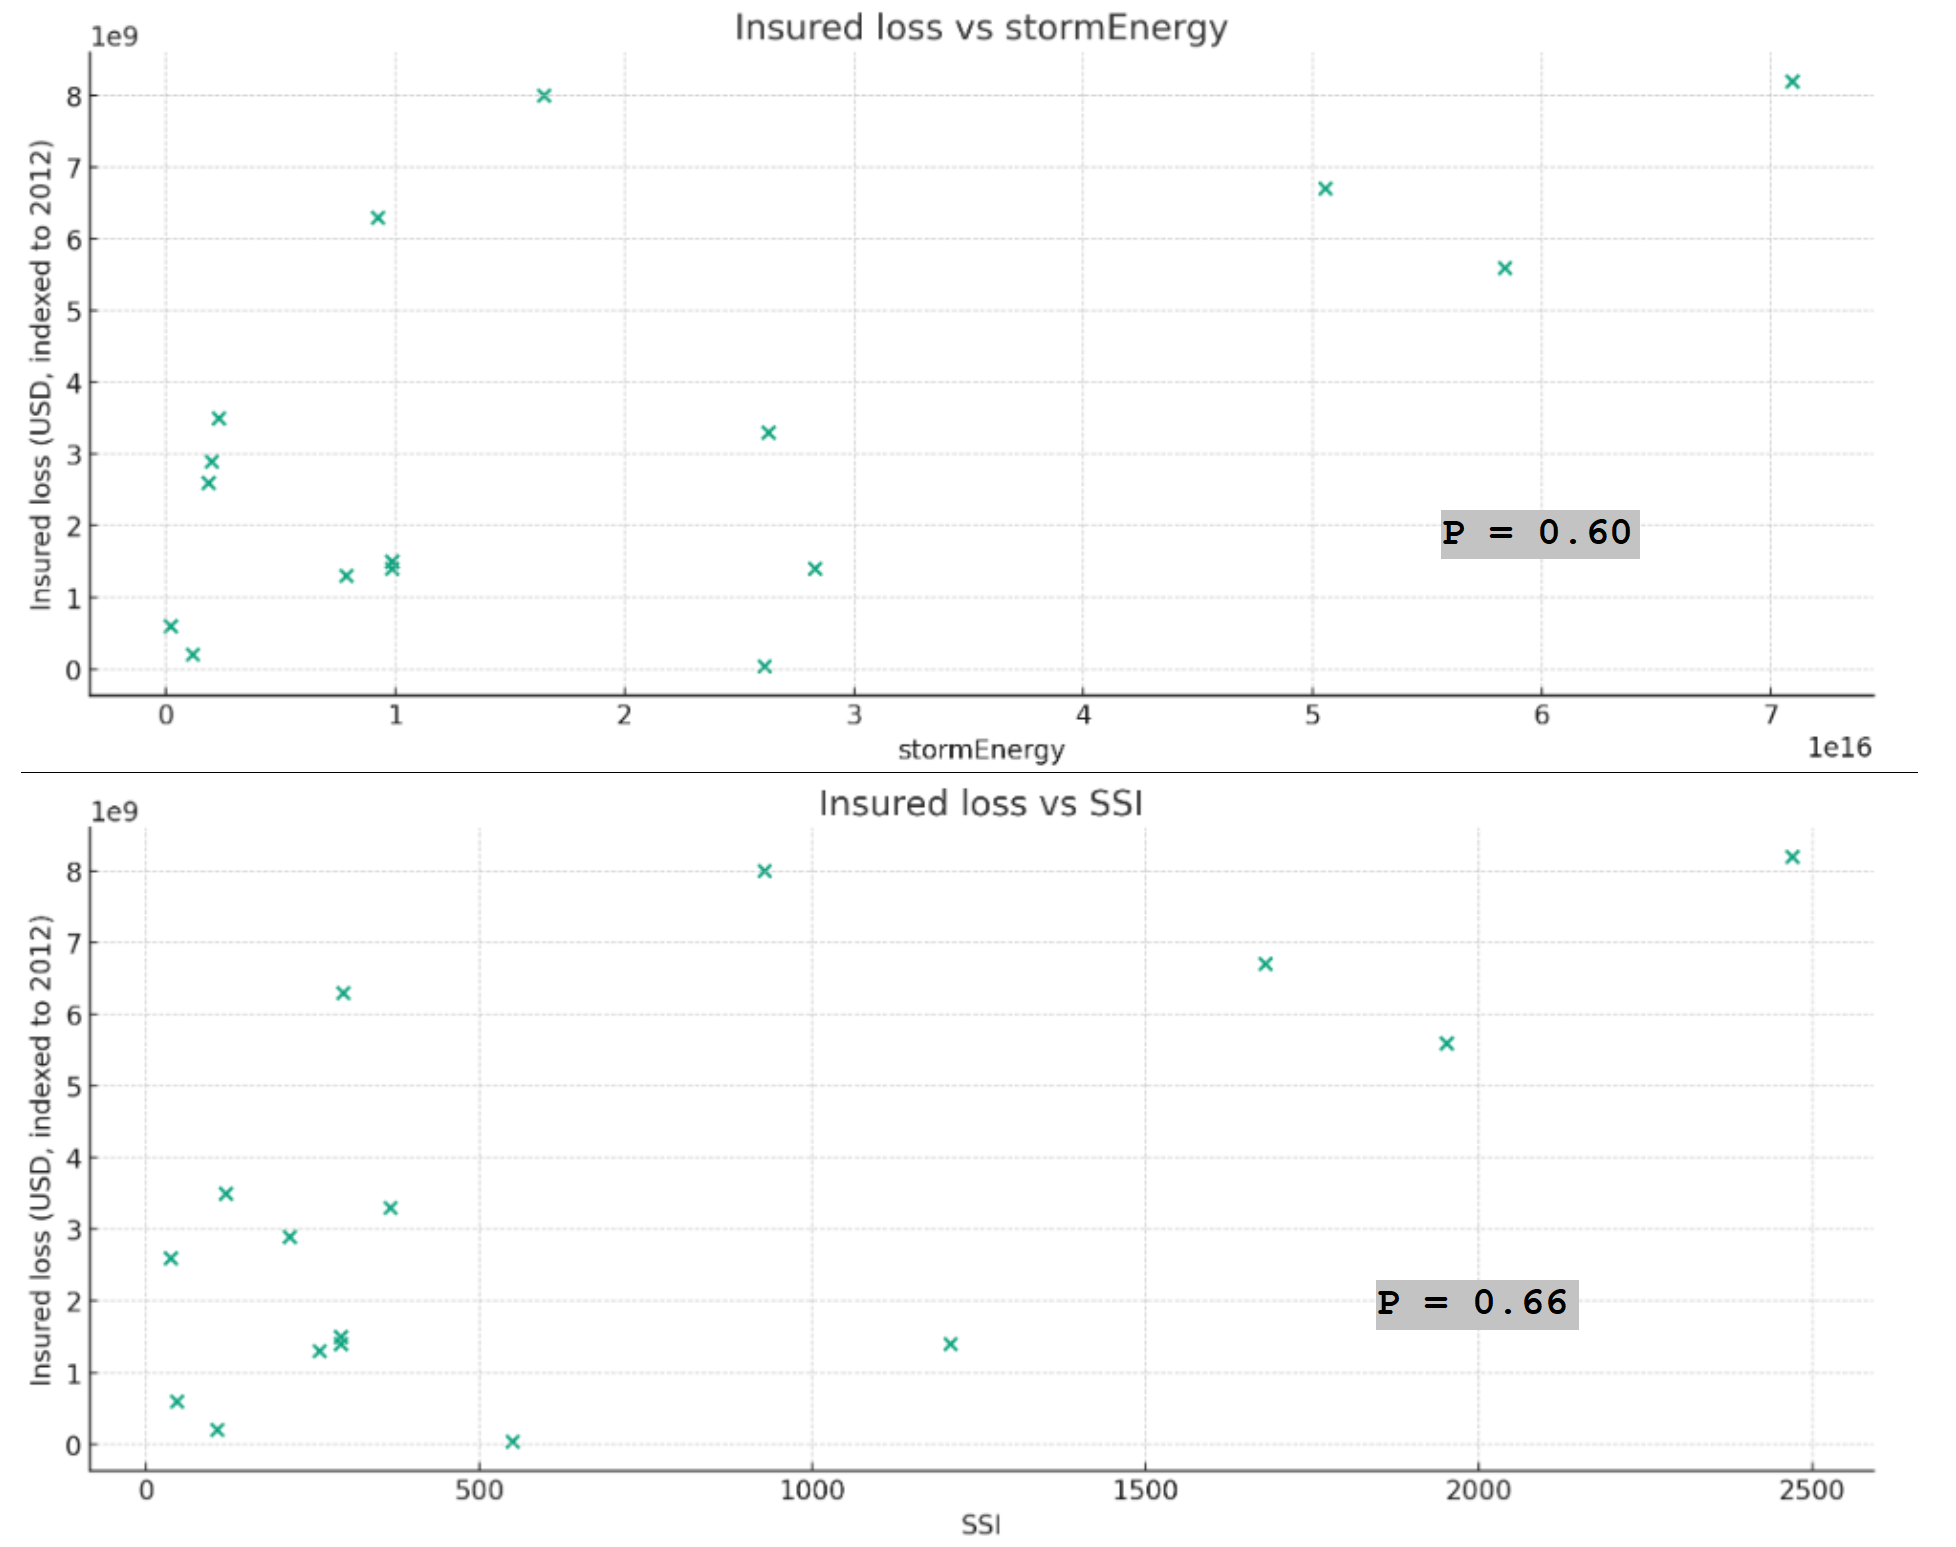
\includegraphics[width=\textwidth]{figures/ssiperformance.png}
            \caption{Performance of the storm energy based SSI method (above) versus an SSI used in industry (below). Both SSI are compared to insurance loss data provided by the Copernicus Extreme Windstorm Catalogue. The P value is reported as 0.60 for the energy method and 0.66 for the industry SSI.}
            \label{fig:scatterSSI}
        \end{figure}

    When estimating the effectiveness of various Storm Severity indices, particularly when they are not designed to measure damage to infrastructure, it is difficult to obtain a confident answer as to which one performs best for a specific measure. In further developing the storm-based SSI, the author hopes to create a detailed and reliable measure which considers all variables of a windstorm and can then be used to benchmark the performance of simpler and less computationally heavy SSIs.